\chapter{実験}
\section{実験目的}
シュミレータ上で,環境を変えて実験を行い,提案手法の有効性の検証を行う.
\section{実験環境}
実験はシミュレータ上で行う.
シミュレータ環境としてオープンソースの
3DロボットシミュレータGazebo\cite{gazebo:online}を用いる.
実験装置として,Fig. \ref{fig::turtlebot3}に示す,turtlebot3\_waffle\cite{turtlebot3:online}へカメラを
3つ追加したモデルを用いる.

\begin{figure}[H]
    \centering
    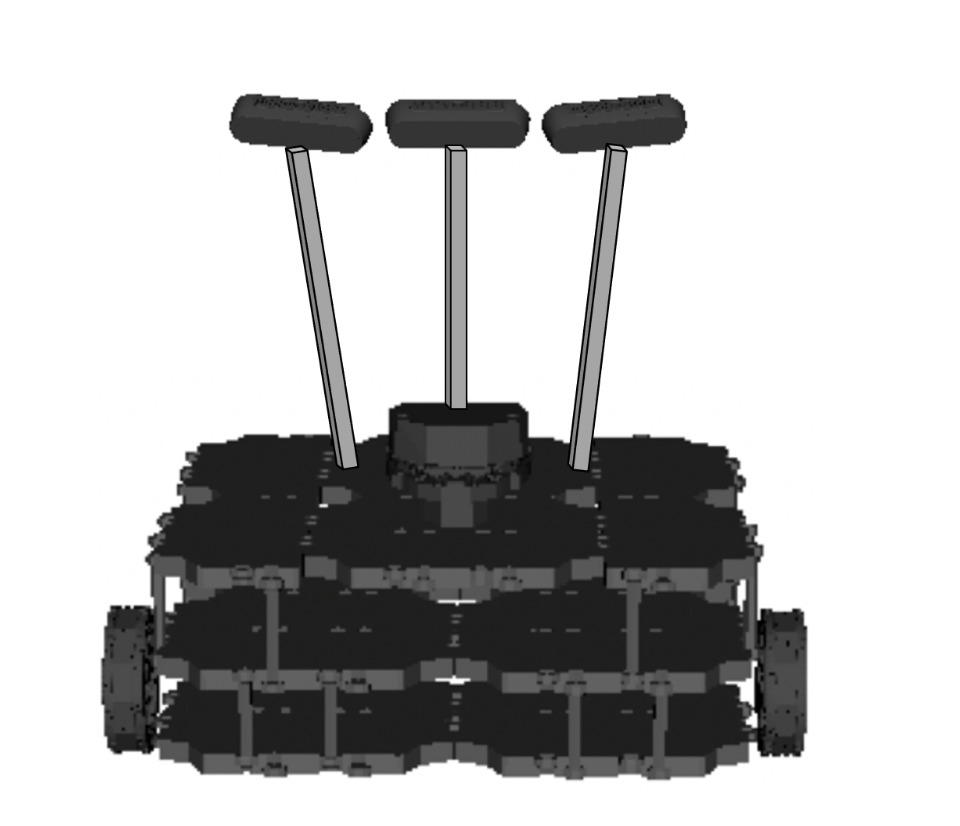
\includegraphics[width = 7cm]{./figs/3_camera.png}
    \caption{Turtlebot3 waffle with 3 cameras}
    \label{fig::turtlebot3}
\end{figure}

\section{実験方法}

実験における手順を下記に示す.
\begin{enumerate}
  \item 設定した経路を学習フェーズで走行し,学習器の訓練(経路の学習)を行う.
  \item テストフェーズへ移行,各経路を設定した回数走行する.
\end{enumerate}
なお,学習器の訓練は「訓練データ (カメラ画像, 目標方向指令) を学習器へ入力し,結果を出力」を 1step とする.
データセットの収集及び,学習器への入力は0.25[s]周期で行う.
また走行に用いる並進速度は0.2[m/s]とする.

\section{実験条件}
実験条件を以下に示す.

テストフェーズにおいて,
\begin{itemize}
  \item 成功:壁に衝突せず, 指定した目標地点へ到達
  \item 失敗:目標方向とは異なった経路を選択, または壁に衝突
\end{itemize}
\newpage
\section{実験1 (十字路を用いた実験)}
\subsection{実験目的}
十字路の単純な環境を用いて,提案手法に基づいて,追加した機能の検証を行う.
\subsection{実験環境}
Fig. \ref{fig::zyuzi}に環境,学習とテストに用いる経路と目標方向を示す.
環境は2.5m幅の十字路の環境を用いる.
この環境へ,ロボットを青で示す初期位置,姿勢で配置する.
経路は下記の手順を6000[step]学習するまで,繰り返し走行する.
なおB,C,DのTarget pointに到達次第,Startの位置へロボットの位置,姿勢を移動させる.
\begin{enumerate}
  \setlength{\parskip}{0cm} % 段落間
  \setlength{\itemsep}{0cm} % 項目間
  \item Start - A - Target point(B)
  \item Start - A - Target point(C)
  \item Start - A - Target point(D)
  \end{enumerate}

\begin{figure}[H]
    \centering
    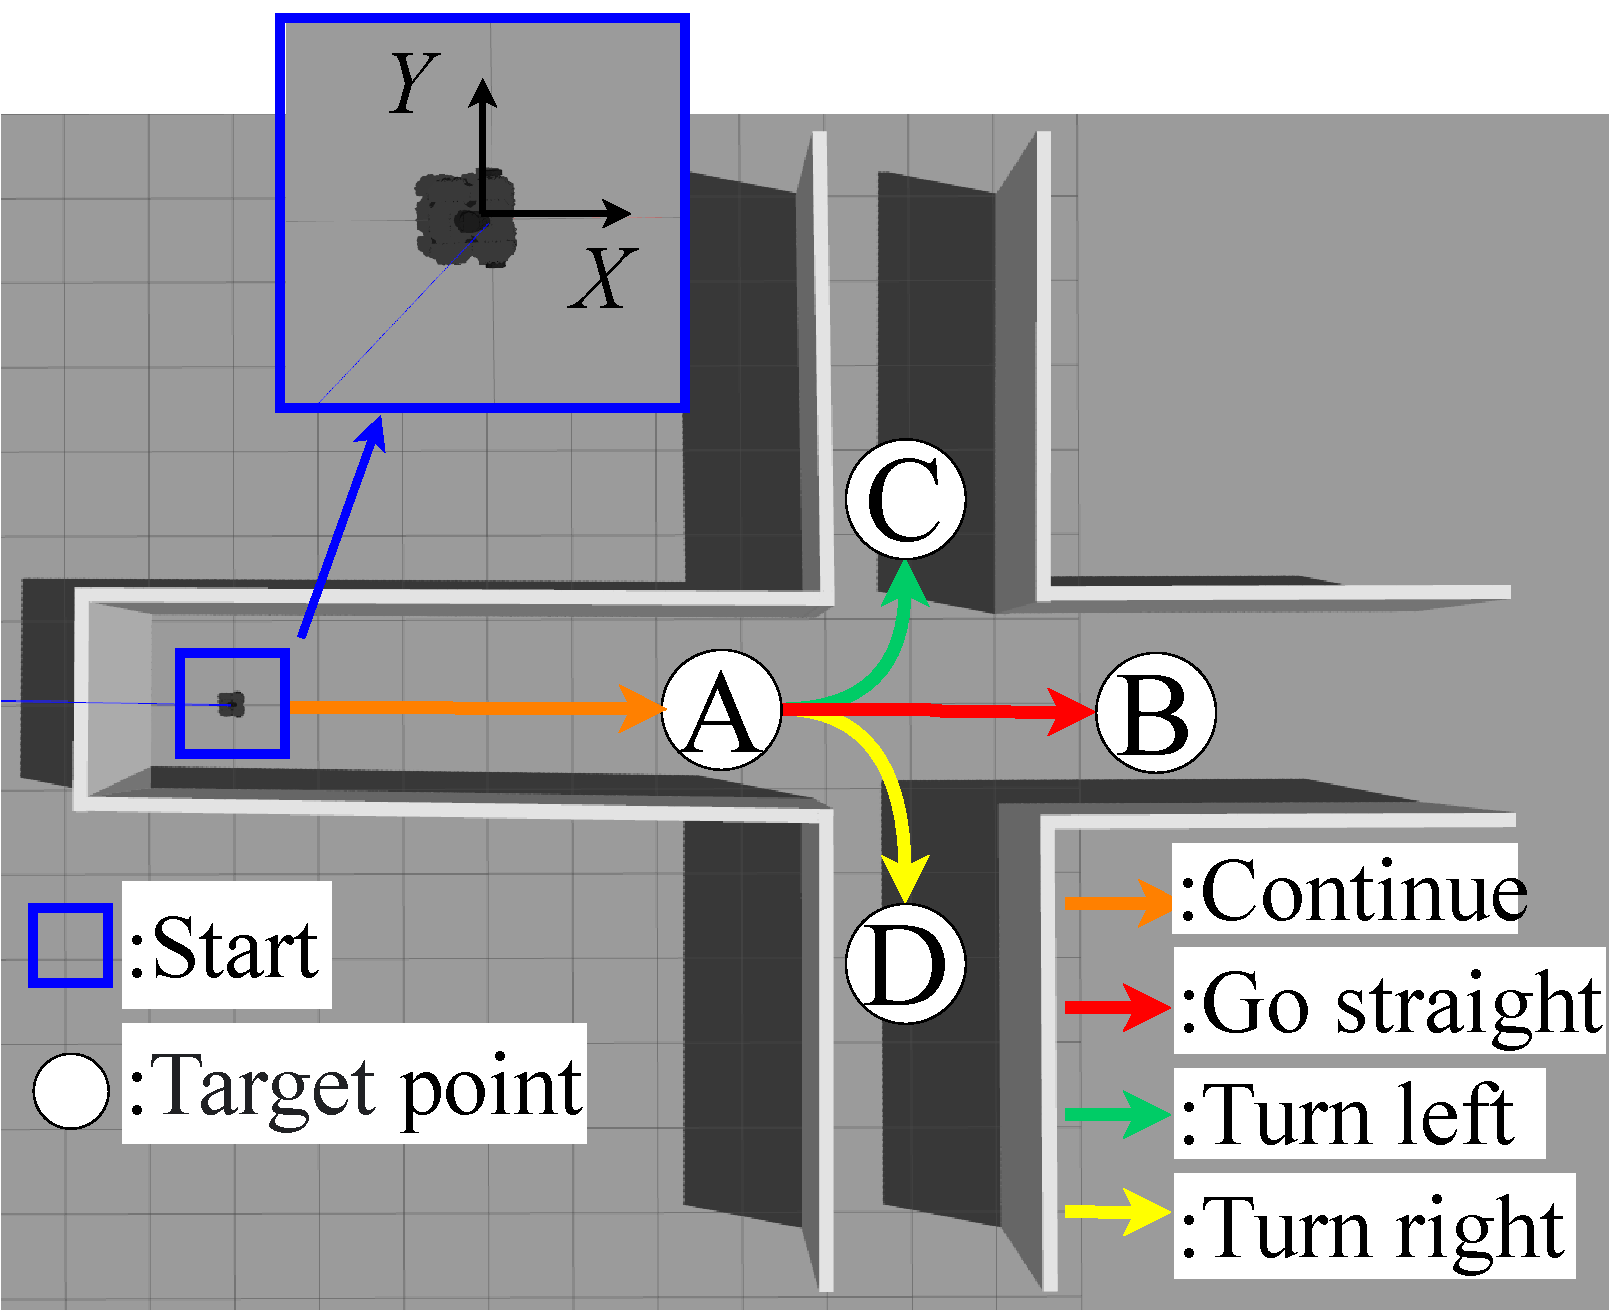
\includegraphics[width = 9.5cm]{./figs/zyuziroute.pdf}
    \caption{Experiment1 course}
    \label{fig::zyuzi}
\end{figure}

% \newpage
% \subsection{学習フェーズでの経路}
% 学習時の経路についてFig. \ref{fig::exp1route}に示す
% Fig内の緑で示す箇所が初期位置,赤で示す円が目標地点である
% 目標地点を1,2,3の順で走行し,到達後初期値点へロボットの位置,姿勢をリセットする.

% \begin{figure}[ht]
%     \centering
%     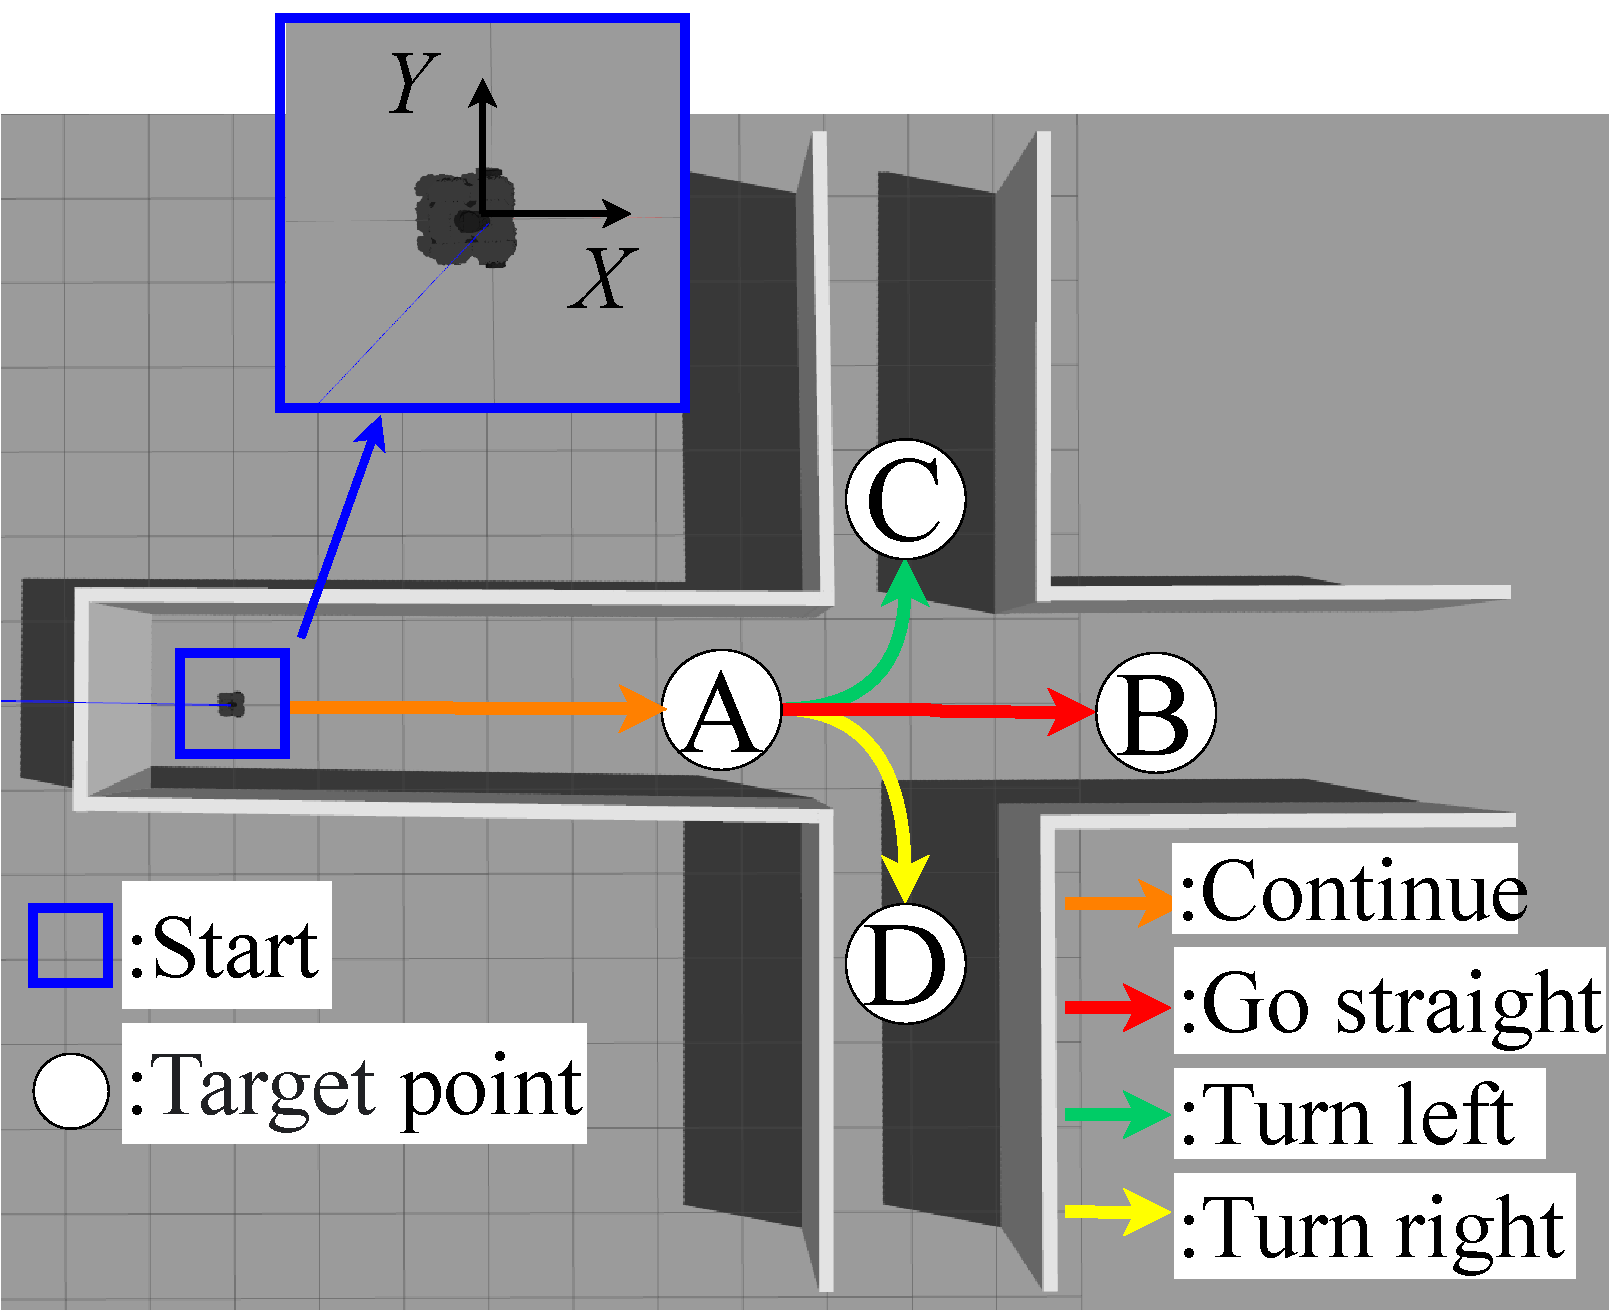
\includegraphics[width = 10cm]{./figs/zyuziroute.pdf}
%     \caption{Route of experiment 1}
%     \label{fig::exp1route}
% \end{figure}

\subsection{評価}
実験の様子をFig. \ref{fig::exp1_view}に示す.
Fig. \ref{exp1_ler_go}, \ref{exp1_ler_left}, \ref{exp1_ler_right}に示す学習フェーズでは,
赤で示した地図ベースの制御器による経路計画へ,追従して走行する様子が確認できた.
また,Fig. \ref{exp1_test_go}, \ref{exp1_test_left}, \ref{exp1_test_right}に示すテストフェーズでは,
目標方向によって,経路を選択する挙動が確認できた.
\begin{figure}[H]
  \begin{tabular}{cc}
    \begin{minipage}[t]{0.5\hsize}
      \centering
      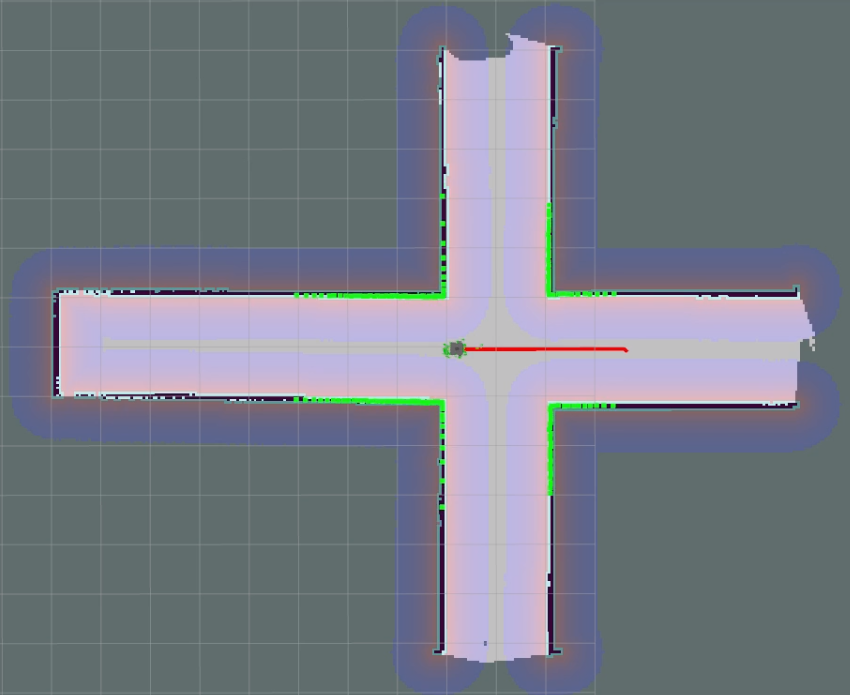
\includegraphics[width=\linewidth]{./figs/zyuzi_ler_go.png}
      \subcaption{Learning phase (target direction:go straight)}
      \label{exp1_ler_go}
    \end{minipage} 
    \begin{minipage}[t]{0.5\hsize}
      \centering
      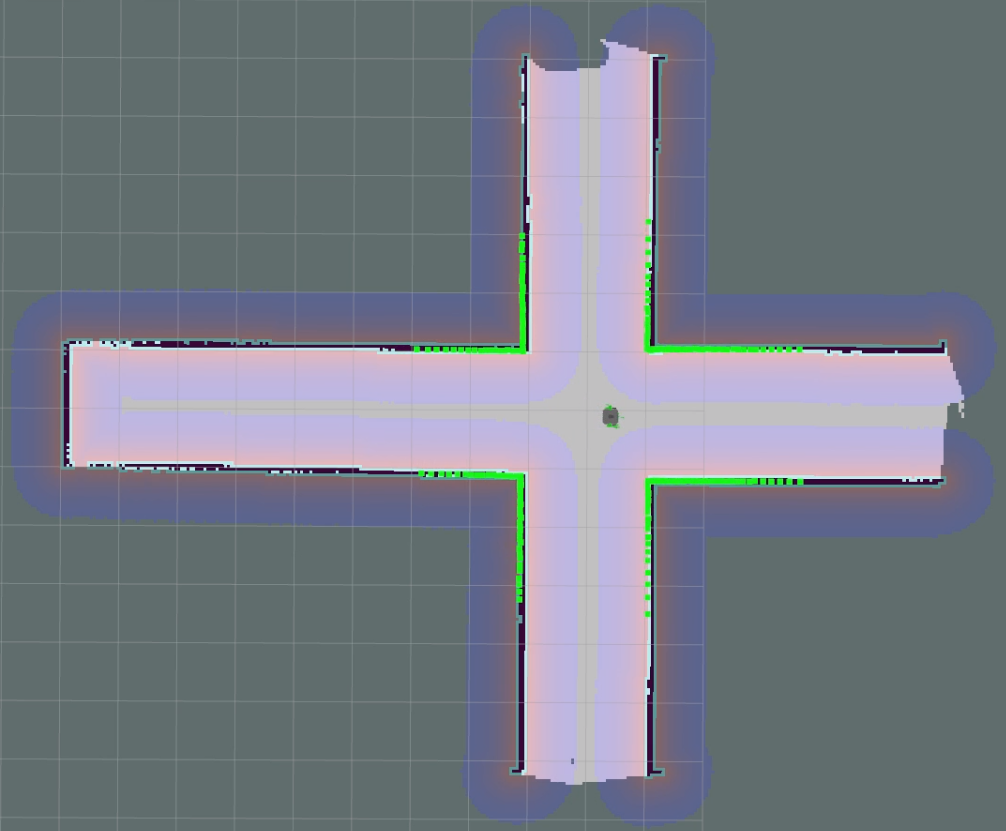
\includegraphics[width=\linewidth]{./figs/zyuzi_test_go.png}
      \subcaption{Test phase (target direction:go straight)}
      \label{exp1_test_go}
    \end{minipage} \\
    \vspace{2.0zh}
    \begin{minipage}[t]{0.5\hsize}
      \centering
      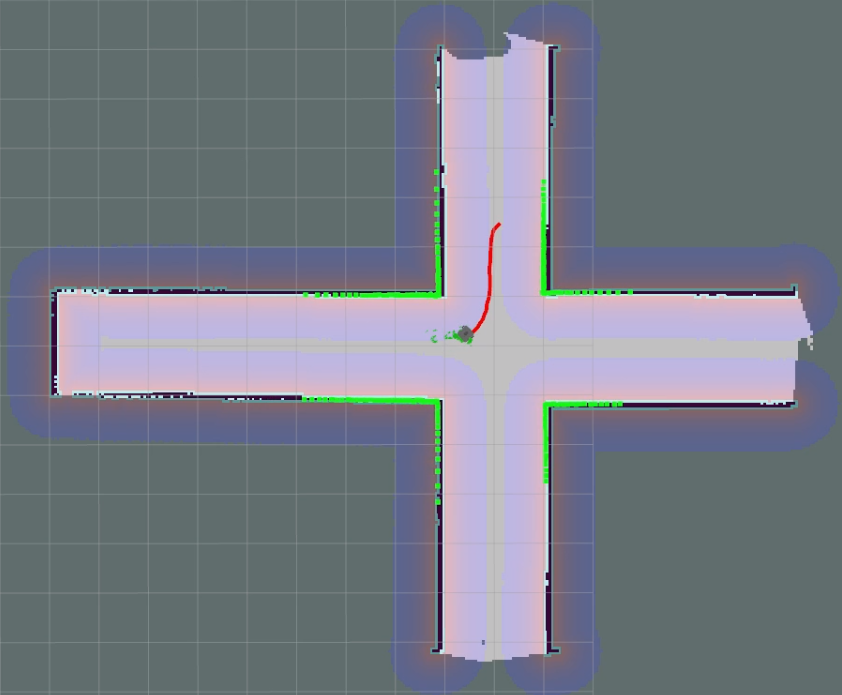
\includegraphics[width=\linewidth]{./figs/zyuzi_ler_left.png}
      \subcaption{Learning phase (target direction:turn left)}
      \label{exp1_ler_left}
    \end{minipage} 
    \begin{minipage}[t]{0.5\hsize}
      \centering
      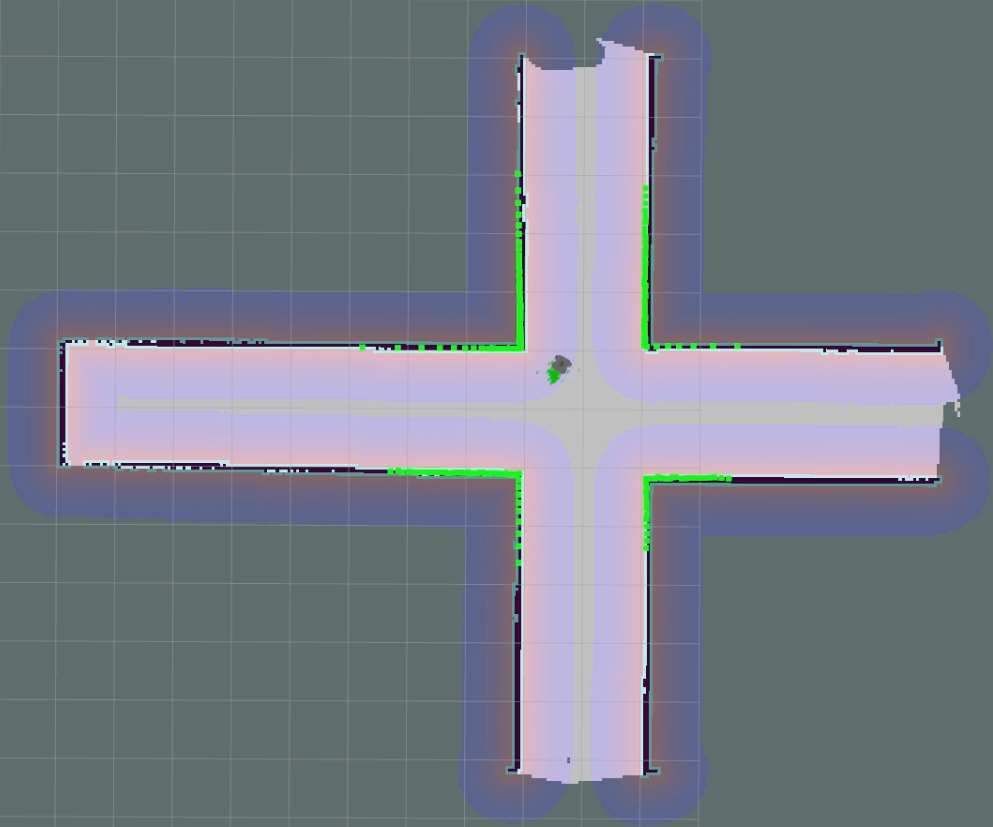
\includegraphics[width=\linewidth]{./figs/zyuzi_test_left.png}
      \subcaption{Test phase (target direction:turn left)}
      \label{exp1_test_left}
    \end{minipage}\\
    \begin{minipage}[t]{0.5\hsize}
      \centering
      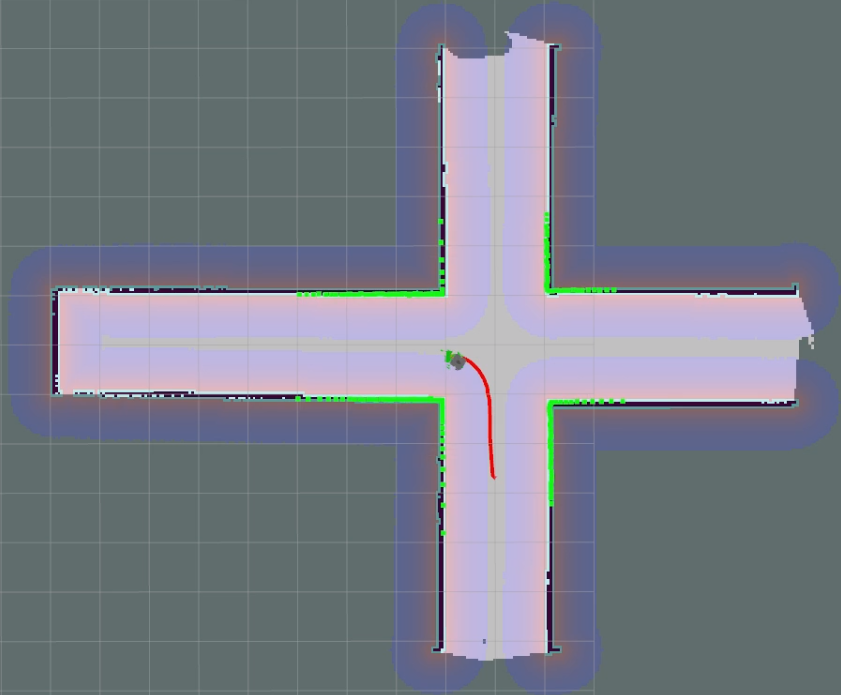
\includegraphics[width=\linewidth]{./figs/zyuzi_ler_right.png}
      \subcaption{Learning phase (target direction:turn right)}
      \label{exp1_ler_right}
    \end{minipage} 
    \begin{minipage}[t]{0.5\hsize}
      \centering
      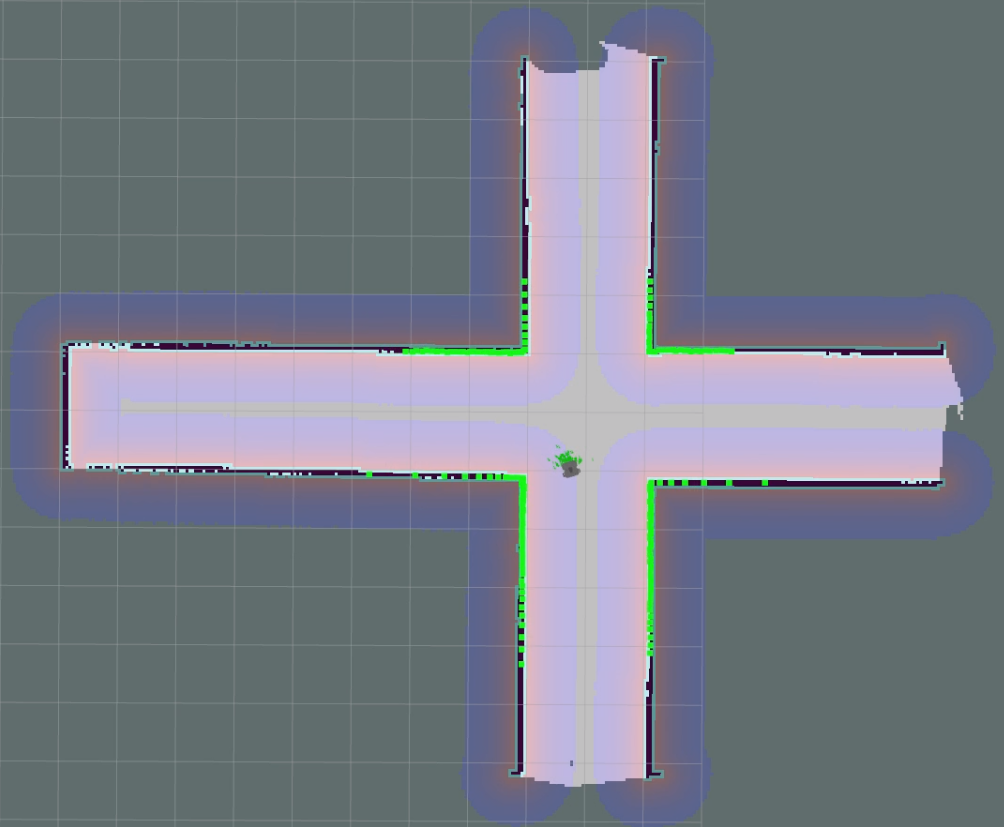
\includegraphics[width=\linewidth]{./figs/zyuzi_test_right.png}
      \subcaption{Test phase (target direction:turn right)}
      \label{exp1_test_right}
    \end{minipage}
  \end{tabular}
   \caption{State of the experiment}
   \label{fig::exp1_view}
\end{figure}
\newpage

\newpage
テストフェーズで,各経路を10回ずつ走行した結果をTable \ref{tb::exp1suc}に示す.
すべての経路において,目標地点へ到達することに成功した.
また,学習フェーズで収集したデータセットをFig. \ref{fig::exp1_result}に示す.
走行回数が多いContinueは突出しているが,それ以外の3つはほぼ同数であることが確認できる.
% \begin{table}[H]
%   \centering
%   \caption{Number of successes experiment 1 point}
%   \begin{tabular}{|c|c|}
%   \hline
%   Point & Number of successes \\ \hline
%   1     & 5/5                  \\ \hline
%   2     & 4/5                  \\ \hline
%   3     & 5/5                  \\ \hline
%   \end{tabular}
  
%   \label{tb::exp1suc}
%   \end{table}
\begin{table}[h]
  \caption{Number of successes experiment1}
  \label{tb::exp1suc}
  \begin{center}
      \vskip 0.5zh
      \begin{tabular}{|c|c|}
          \hline
          Route & Number of successes\\ \hline
          % Start - A (continue) & $10/10$ \\ \hline
          Start - A - B  & $10/10$ \\ \hline
          Start - A - C  & $10/10$ \\ \hline
          Start - A - D  & $10/10$ \\ \hline
      \end{tabular}
  \end{center}
\end{table}

\begin{figure}[ht]
  \centering
  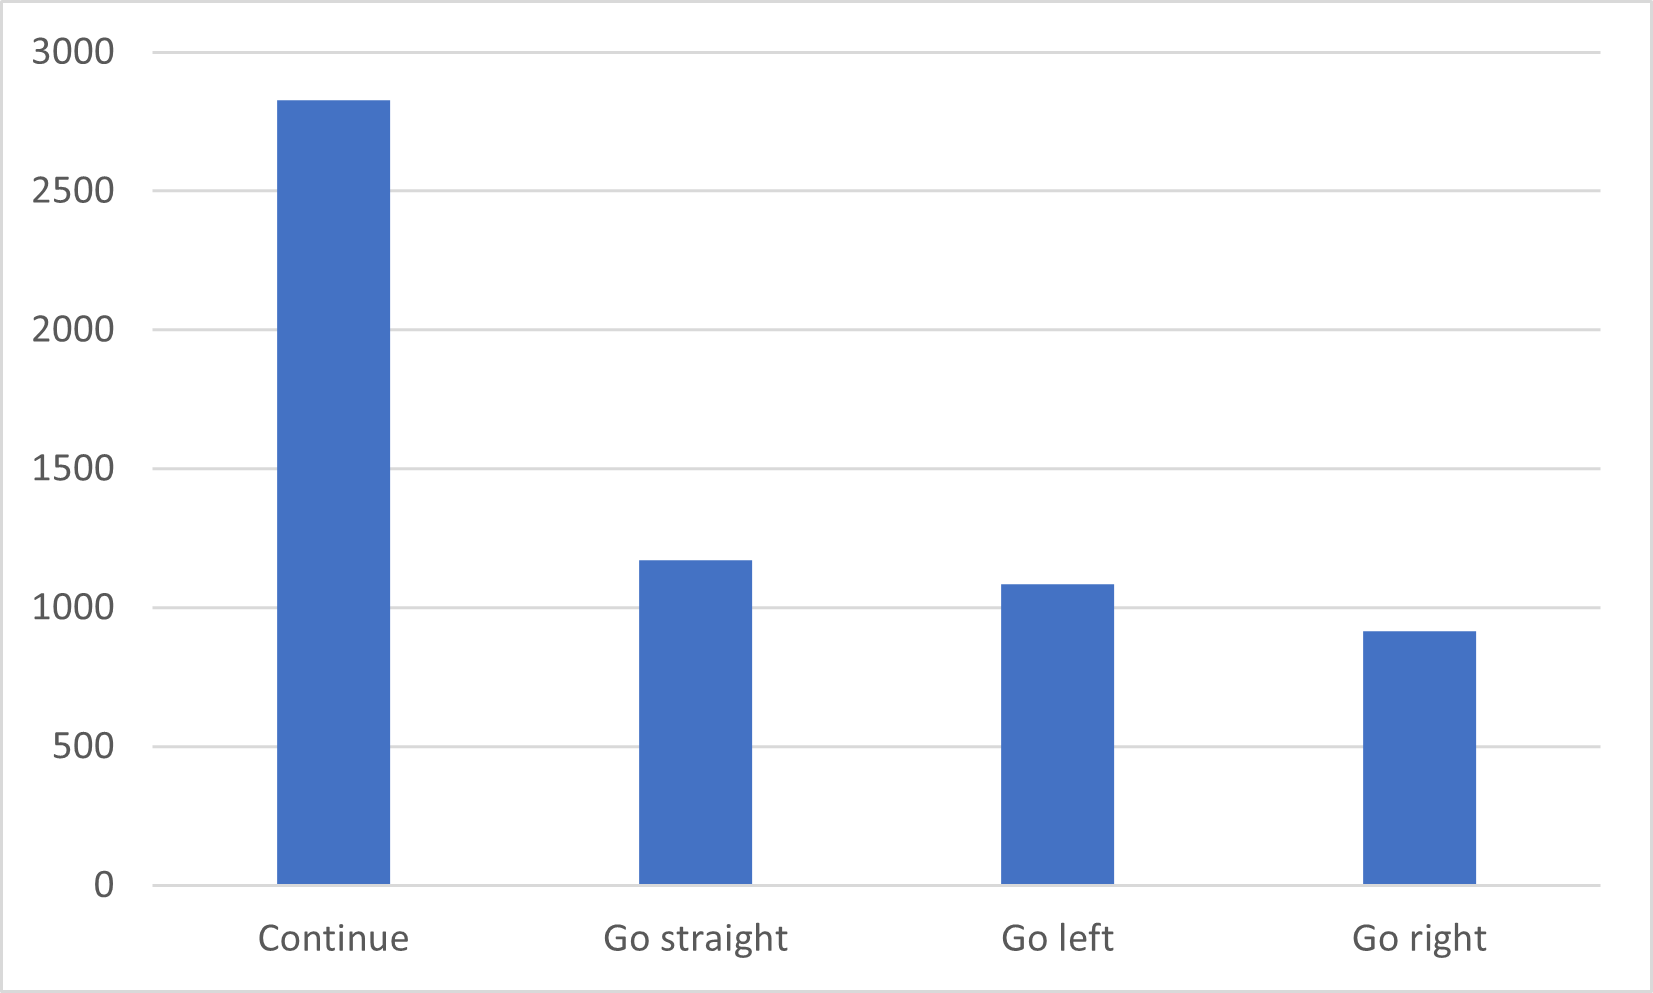
\includegraphics[width = 10cm]{./figs/exp1_result.png}
  \caption{Experiment1 dataset}
  \label{fig::exp1_result}
\end{figure}

\newpage
\section{実験2 (8の字コースを用いた実験)}
\subsection{実験目的}
実験1で用いた1つの十字路から環境を拡張し,
複雑な経路でも経路選択できるかを検証する.
% 提案手法を用いて,分岐路においてコマンドによってルートの変更が可能であるかさらなる検証を行う.
\subsection{実験環境}
Fig. \ref{fig::hatinozi}に示す.縦8[m]×横12[m]で道幅が2.5[m]の8の字型の環境を用いる.
この環境へロボットを青で示す初期位置,姿勢で配置する.
\begin{figure}[H]
    \centering
    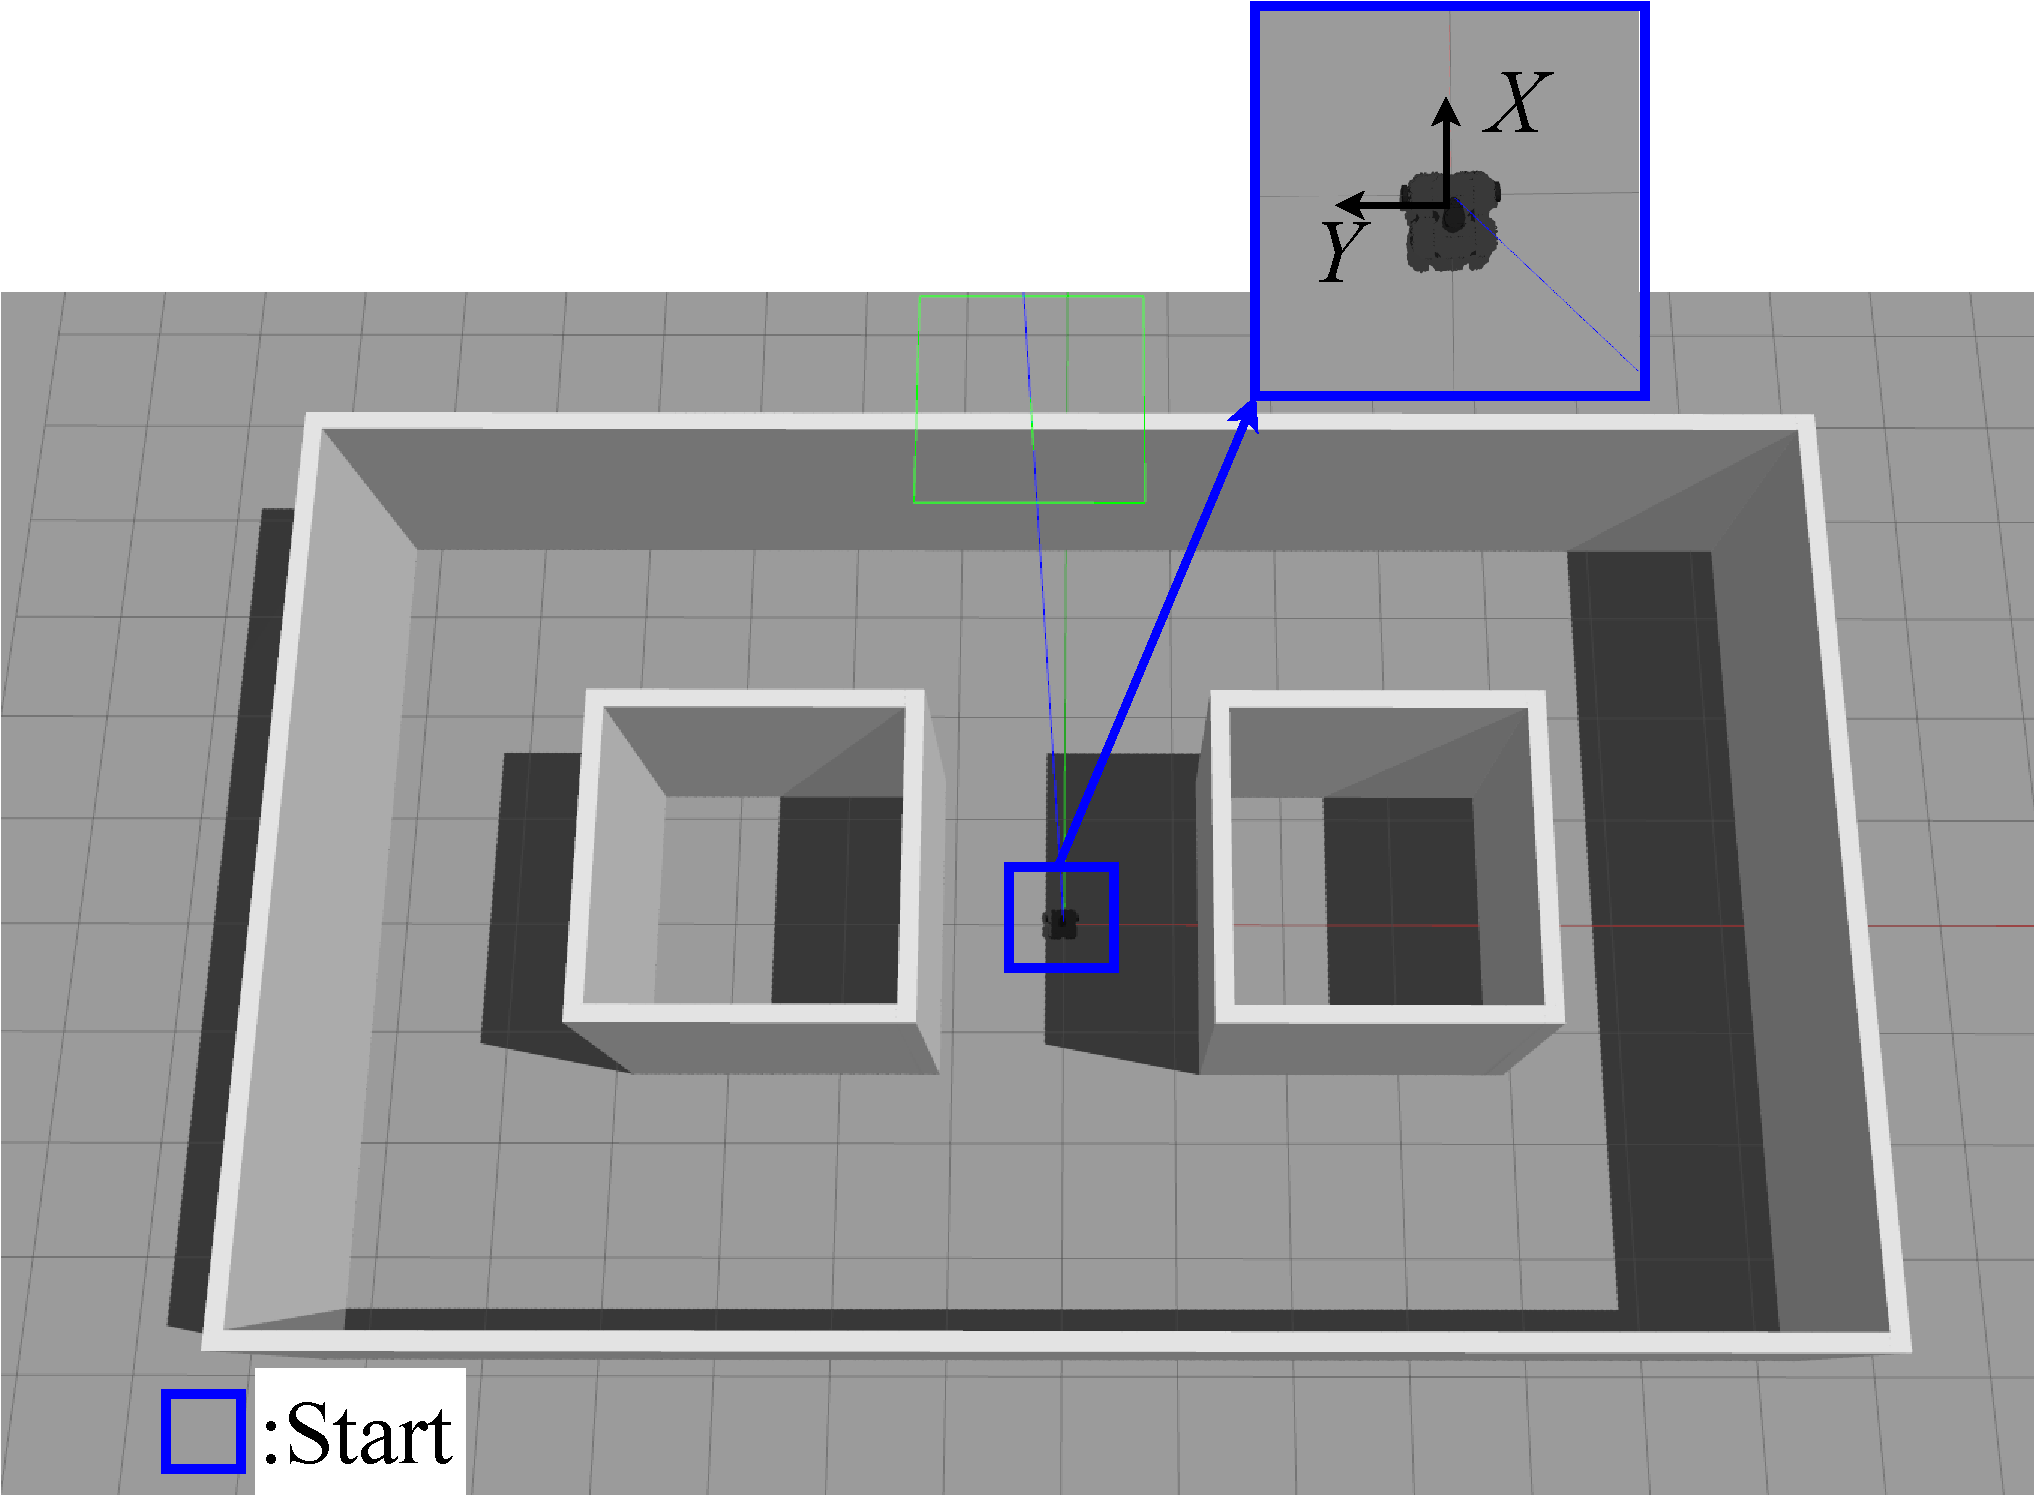
\includegraphics[width = 12cm]{./figs/coli.pdf}
    \caption{Experiment2 course}
    \label{fig::hatinozi}
\end{figure}

\newpage
Fig. \ref{fig::exp2route}に実験に用いる経路と,学習とテストで用いる目標方向を示す.
これらの環境を網羅するような経路を,
Route A-Fの順で60000[step]学習するまで,繰り返し走行する.
\begin{figure}[H]
    \begin{tabular}{cc}
      \begin{minipage}[t]{0.5\hsize}
        \centering
        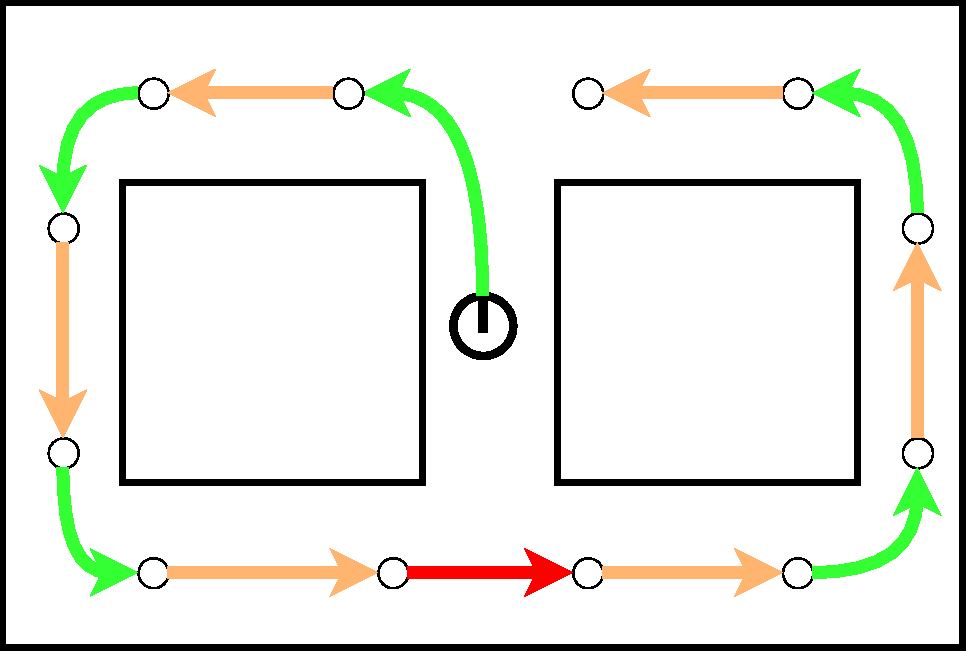
\includegraphics[keepaspectratio, scale=0.38]{./figs/8nozi_route-r1.pdf}
        \subcaption{Route A}
        \label{exp2route1}
      \end{minipage} 
      \begin{minipage}[t]{0.5\hsize}
        \centering
        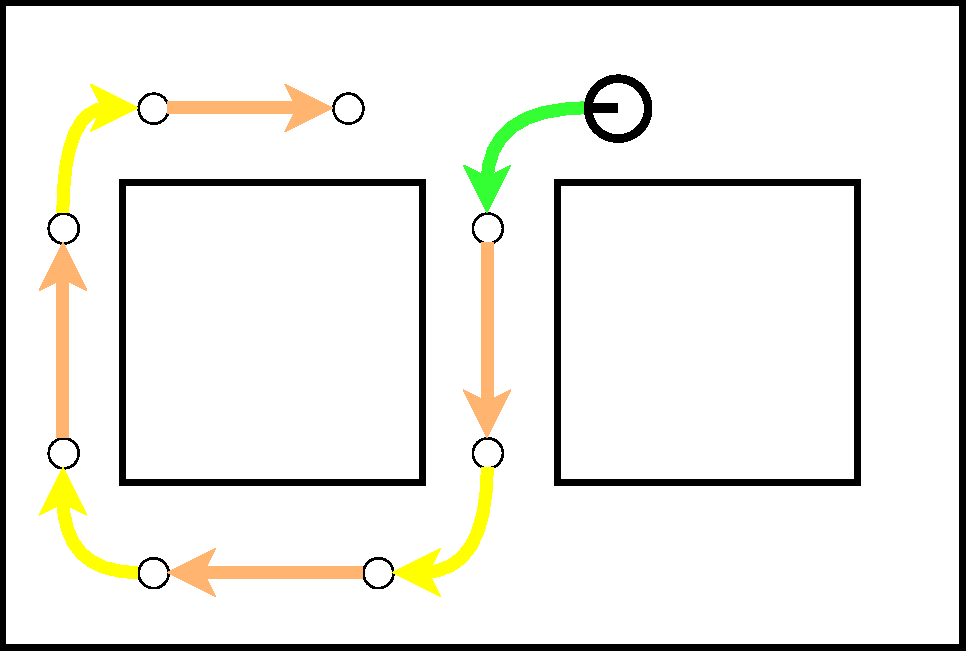
\includegraphics[keepaspectratio, scale=0.38]{./figs/8nozi_route-r2.pdf}
        \subcaption{Route B}
        \label{exp2route2}
      \end{minipage} \\
      \vspace{2.0zh}
      \begin{minipage}[t]{0.5\hsize}
        \centering
        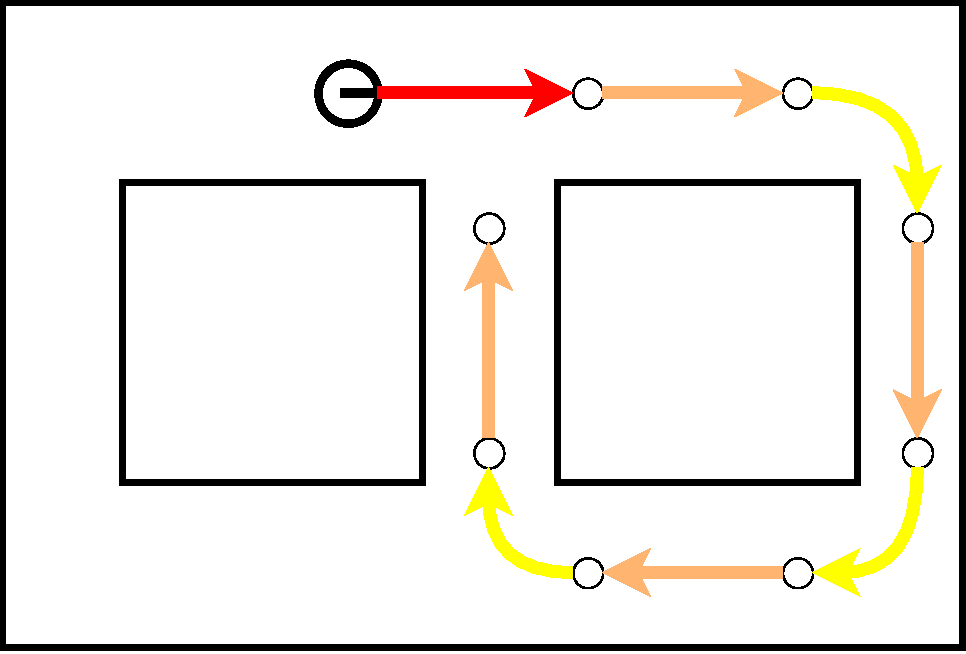
\includegraphics[keepaspectratio, scale=0.38]{./figs/8nozi_route-r3.pdf}
        \subcaption{Route C}
        \label{exp2route3}
      \end{minipage} 
      \begin{minipage}[t]{0.5\hsize}
        \centering
        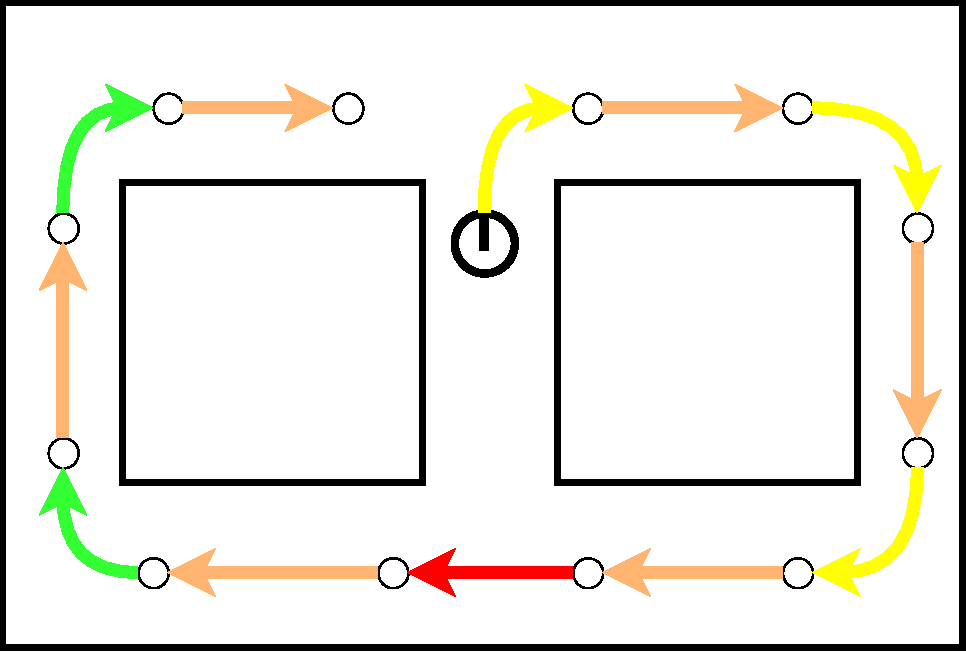
\includegraphics[keepaspectratio, scale=0.38]{./figs/8nozi_route-r4.pdf}
        \subcaption{Route D}
        \label{exp2route4}
      \end{minipage}\\

      \begin{minipage}[t]{0.5\hsize}
        \centering
        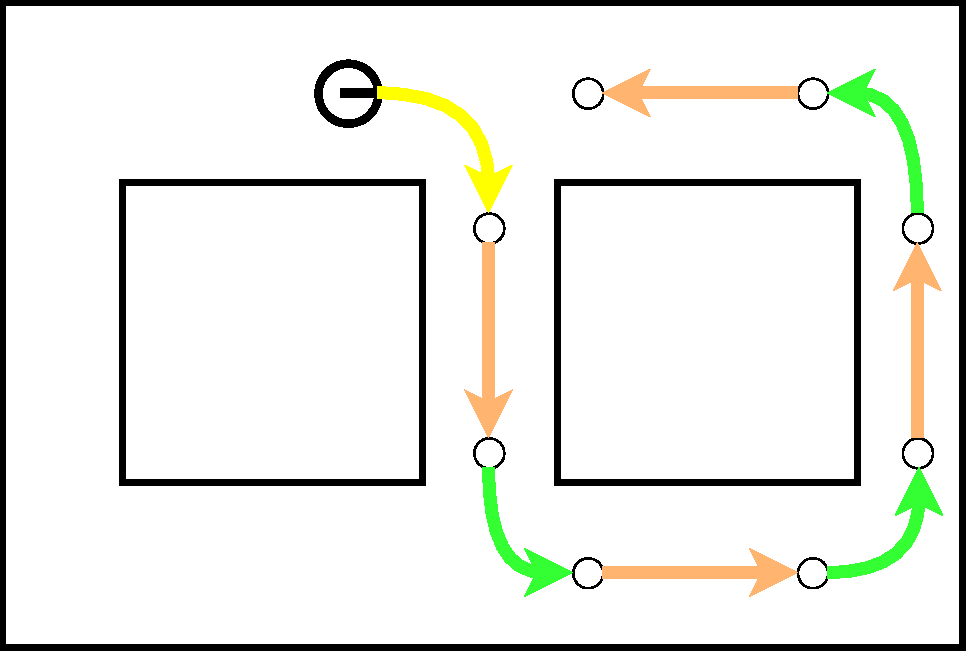
\includegraphics[keepaspectratio, scale=0.38]{./figs/8nozi_route-r5.pdf}
        \subcaption{Route E}
        \label{exp2route5}
      \end{minipage} 
      \begin{minipage}[t]{0.5\hsize}
        \centering
        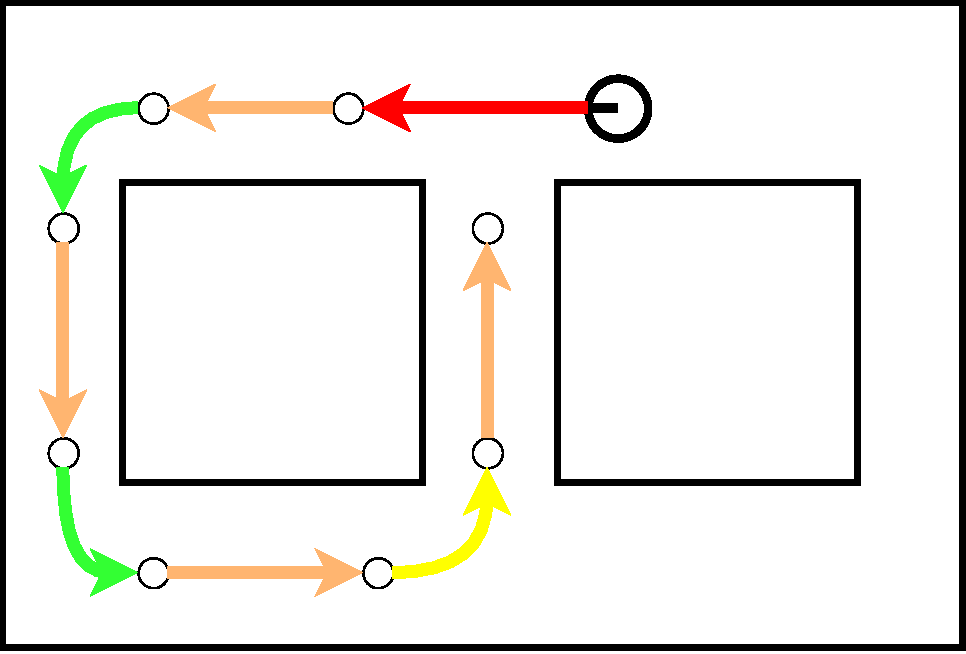
\includegraphics[keepaspectratio, scale=0.38]{./figs/8nozi_route-r6.pdf}
        \subcaption{Route F}
        \label{exp2route6}
      \end{minipage}
    \end{tabular}
    \begin{figure}[h]
      \centering
      
\includegraphics[width = 10cm]{./figs/8nizi_cap.pdf}
  \end{figure}
     \caption{Experiment 2 route}
     \label{fig::exp2route}
  \end{figure}
  
\newpage
\subsection{評価}
実験の様子をFig. \ref{fig::exp1_view}に示す.
Fig. \ref{exp1_ler_go}, \ref{exp1_ler_left}, \ref{exp1_ler_right}に示す学習フェーズでは,
赤で示した地図ベースの制御器による経路計画へ,追従するように走行する様子が確認できる.
また,Fig. \ref{exp1_test_go}, \ref{exp1_test_left}, \ref{exp1_test_right}に示すテストフェーズにおいて,
同一の分岐路で,目標方向により経路を選択する挙動が確認できる.
\begin{figure}[h]
  \begin{tabular}{cc}
    \begin{minipage}[t]{0.5\hsize}
      \centering
      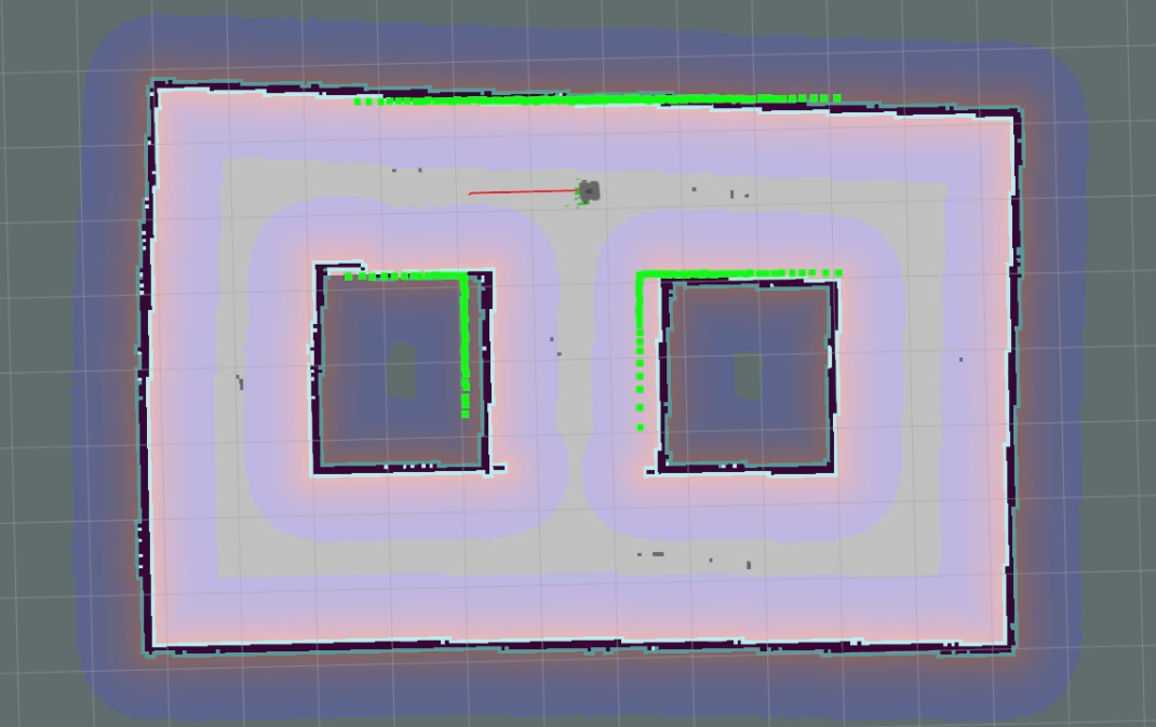
\includegraphics[height=4.3cm]{./figs/coli_ler_go.png}
      \subcaption{Learning phase (target direction:go straight)}
      \label{exp2_ler_go}
    \end{minipage} 
    \begin{minipage}[t]{0.5\hsize}
      \centering
      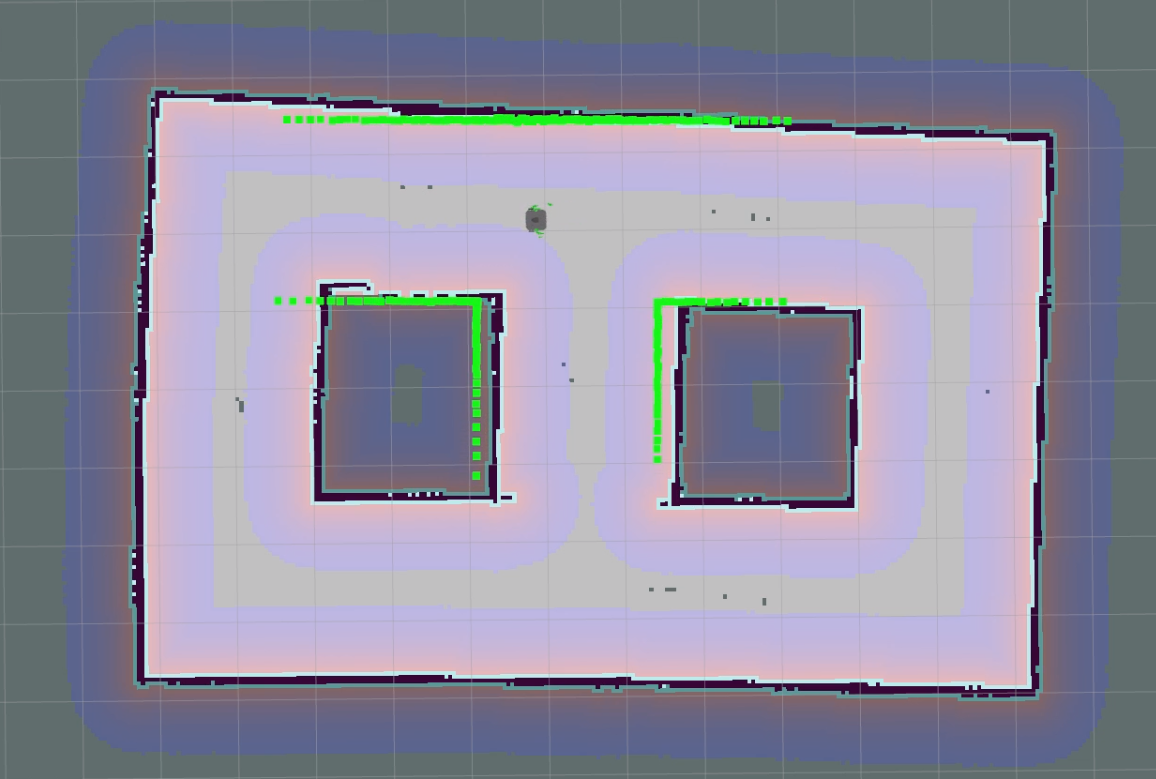
\includegraphics[height=4.3cm]{./figs/coli_test_go.png}
      \subcaption{Test phase (target direction:go straight)}
      \label{exp2_test_go}
    \end{minipage} \\
    \begin{minipage}[t]{0.5\hsize}
      \centering
      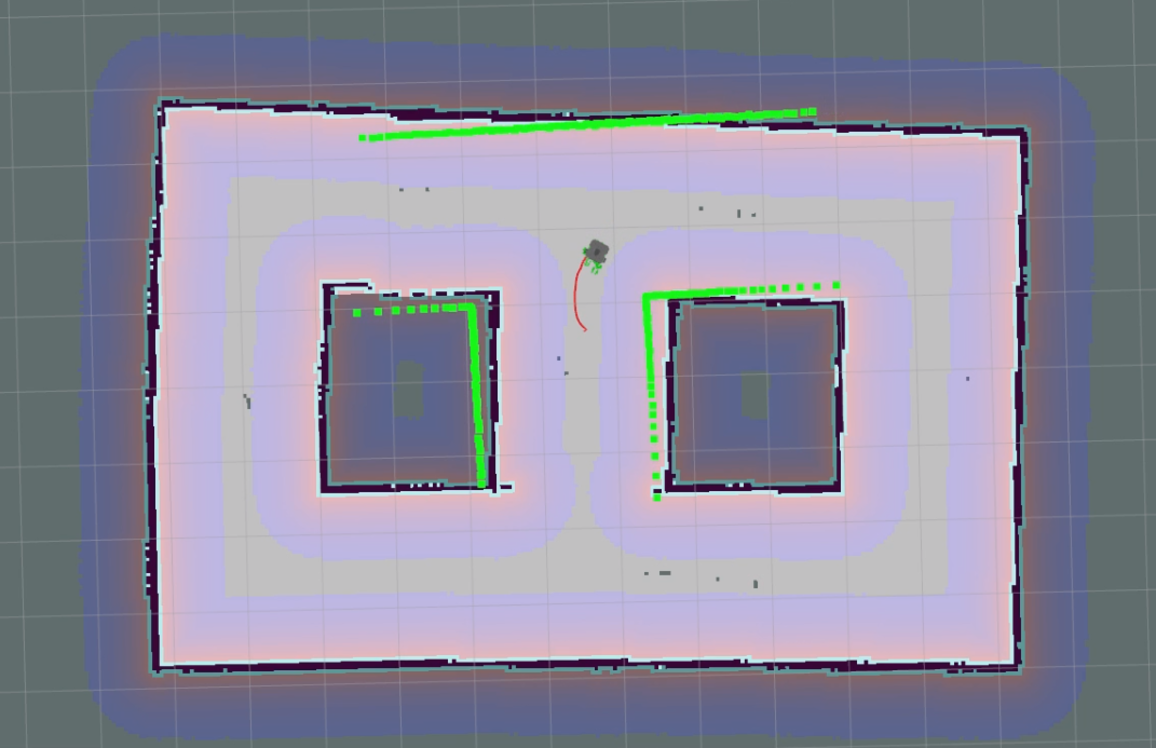
\includegraphics[height=4.4cm]{./figs/coli_ler_left.png}
      \subcaption{Learning phase (target direction:turn left)}
      \label{exp2_ler_left}
    \end{minipage} 
    \begin{minipage}[t]{0.5\hsize}
      \centering
      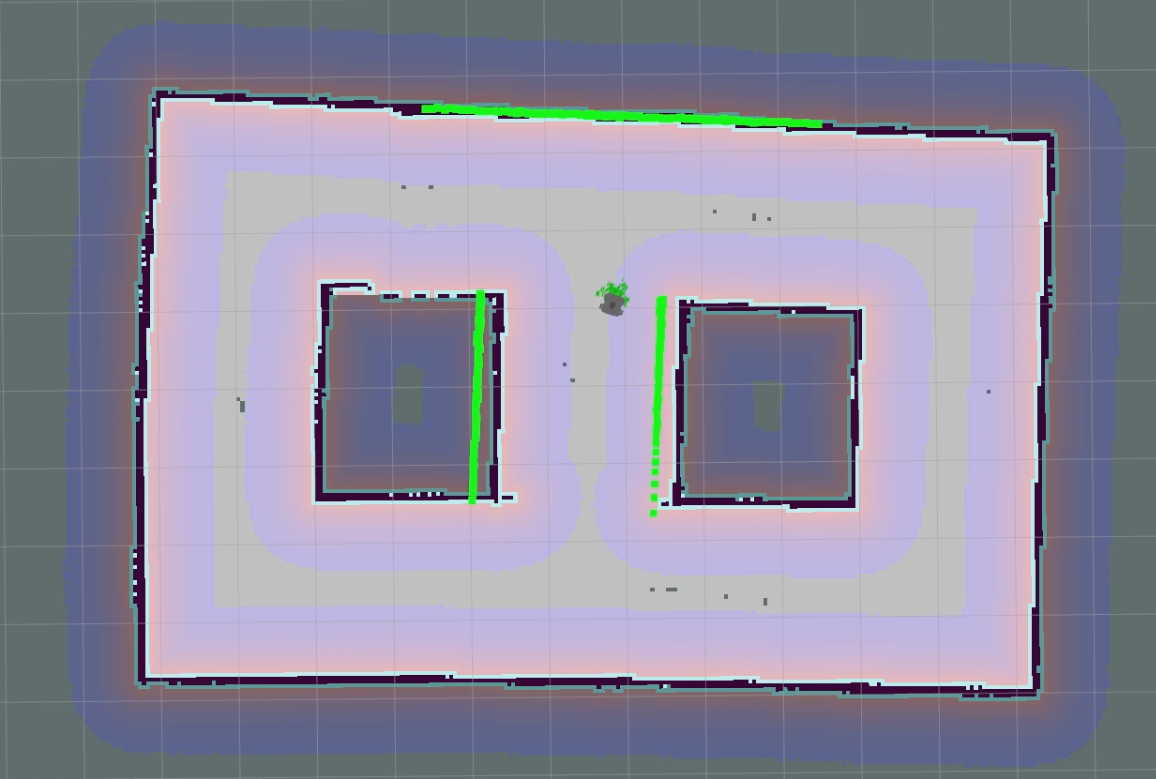
\includegraphics[height=4.4cm]{./figs/coli_test_left.png}
      \subcaption{Test phase (target direction:go turn left)}
      \label{exp2_test_left}
    \end{minipage} \\
  \end{tabular}
   \caption{State of the experiment2}
   \label{fig::exp2_view}
\end{figure}
\newpage
テストフェーズで,経路をランダムに60回走行を行った結果をTable \ref{tb::exp2suc}に示す.
結果として経路を約8割走行することに成功した.
また,学習フェーズで収集した目標方向指令のデータセットをFig. \ref{fig::exp2_result}に示す.
Go left,Go rightはほぼ同数であるが,Go straightは約半分以下となった.
しかし,Go straightを用いた,経路の選択は問題なく行うことができた.
これは,Go straightが学習する角速度が,Continueと類似しているからだと考えられる.
  \begin{table}[htb]
    \centering
    \caption{Number of successes experiment2}
    \begin{tabular}{|c|c|}
    \hline
    Route & Number of successes \\ \hline
    A-F     & 50/60                  \\ \hline
    \end{tabular}
    \label{tb::exp2suc}
    \vspace{2zh}
    \end{table} 
    \begin{figure}[ht]
      \centering
      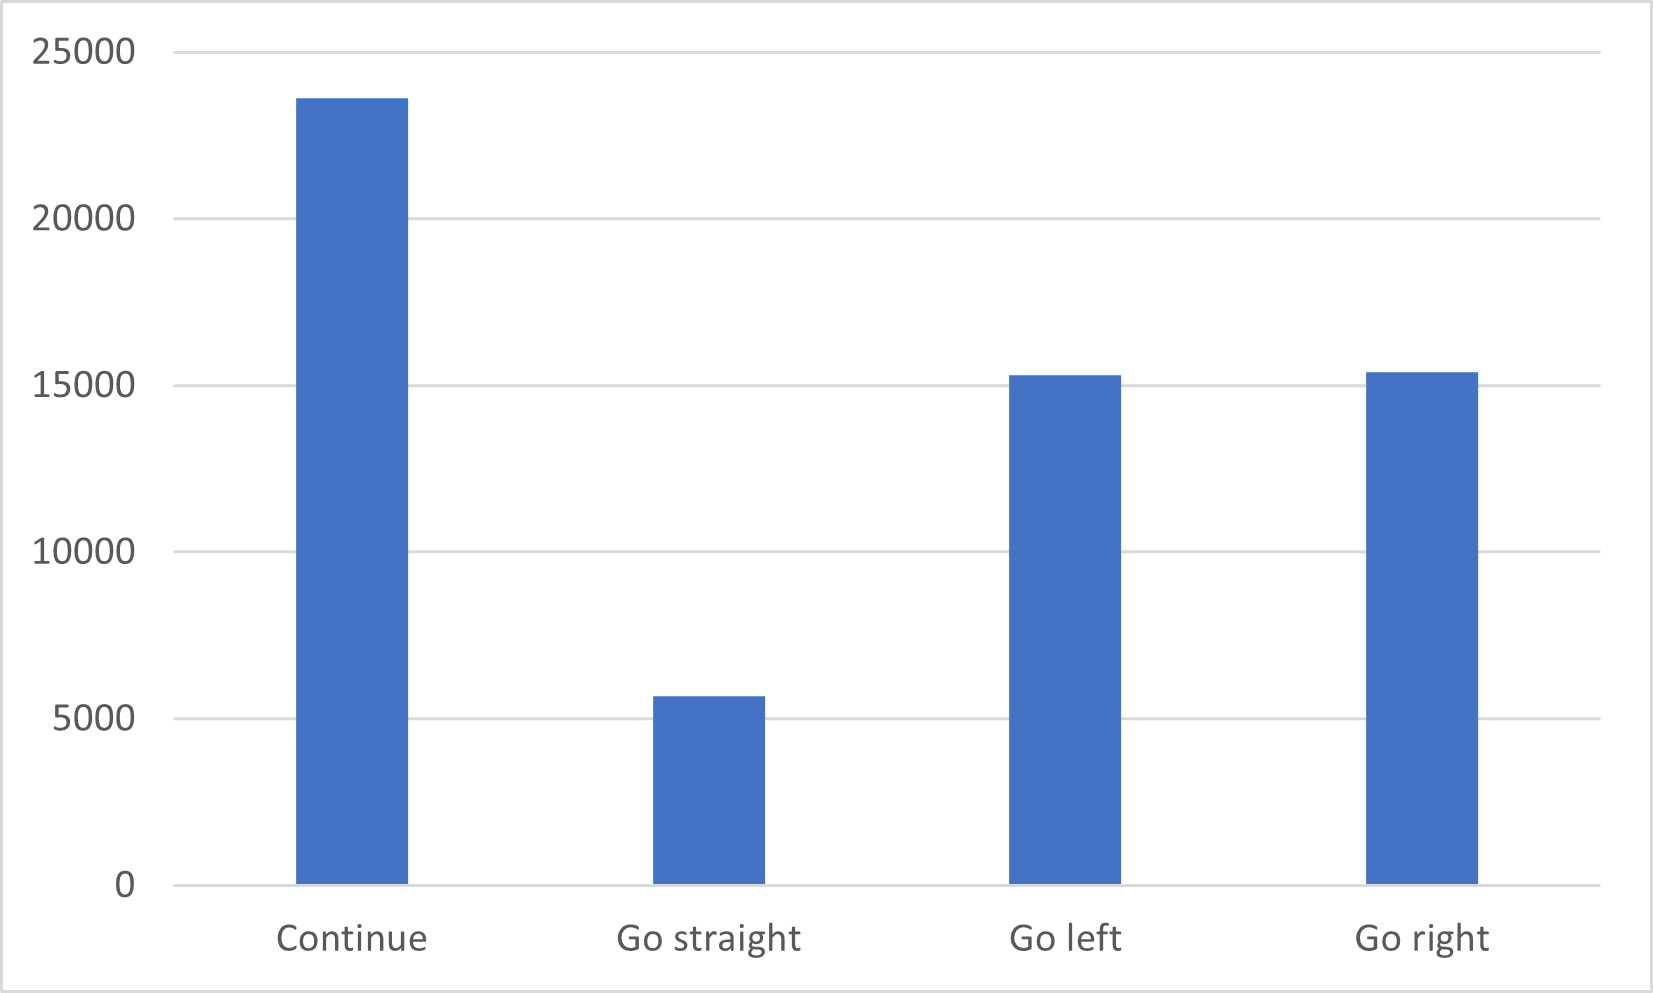
\includegraphics[width = 10cm]{./figs/exp2_result.png}
      \caption{Experiment2 dataset}
      \label{fig::exp2_result}
    \end{figure}